%%% Local Variables:
%%% mode: latex
%%% TeX-master: "IS1apuntes"
%%% End:

\textbf{Ingenería del Software} (\emph{IEEE}) La aplicación de un
enfoque sistemático, disciplinado y cuantificable al desarrollo,
operación y mantenimiento de \emph{software}.\par
Las \textbf{Ciencias de la Computación} se preocupa de los fundamentos
de la teoría; mientras que la Ingeniería del Software de los aspectos
prácticos.\par
La \textbf{Ingeniería del Software} estudia los \textbf{productos}
producidos (ejecutables, módulos, sistemas, liberías...) y los
\textbf{procesos} usados para producir esos productos.

\section{La crisis del Software}
\label{sec:crisis}

Los principales problemas que hay detrás de la crisis del Software
son:
\begin{itemize}[noitemsep]
\item El incremento en el tamaño y la complejidad.
\item Los sobrecostes.
\item Fallos en el diseño.
\item Mal mantenimiento.
\item Herramientas no solo de programación.
\end{itemize}

Pero desde un enfoque más moderno, también se aprecian otros tipos de
problemas:

\begin{itemize}[noitemsep]
\item Falta de robustez en el Software para componentes críticos o de
  los que somos dependientes.
\item Excesiva complejidad en el Software como para entenderlo y
  comprenderlo.
\item Exigencia de cambiar rápidamente.
\end{itemize}

Frente a esto, desde la Ingeniería del Software se plantea la mejora
en las metodologías y el uso de lenguajes de alto nivel (mayor
abstacción).

Tras el intento de solucinar estos problemas, el concepto de Ingeniería
del Software se redefine en:\par

\begin{center}
\textit{Disciplina que tiene como objetivo la producción de
  Software libre de errores, sin retrasos y dentro del presupuesto;
  satisfaciendo las necesidades del cliente}  
\end{center}

\section{Costes en la Ingeniería del Software}
\label{sec:costes}
\index{costes}
En cuanto a la realización del producto, aproximadamente el 60\% del
coste es en desarrollo, y el 50\% en pruebas (test). Sin embargo,
con el uso del software, los gastos de mantenimiento superan a los del
desarrollo.

\begin{figure}[h]
  \caption[Coste - Metodología]{Distribución del coste según
    metodología}
  \pgfplotsset{testbar/.style={
      xbar stacked, area style,
      width=12cm,
      axis y line*= none, axis x line*= bottom,
      xmajorgrids = true,
      xmin=0,xmax=100,
      ytick = data,
      yticklabels = {},
      point meta = x,
      tick align = outside, xtick pos = left,
      bar width=6mm, y=8mm,
      enlarge y limits={abs=0.625},% 0.5 + 0.5*(y - bar width)/y [TeX.sx #47995]
      nodes near coords,
      every node near coord/.append style={rotate=-90,font=\small, left,shift={(axis direction cs:-3,0)}}
    }}
  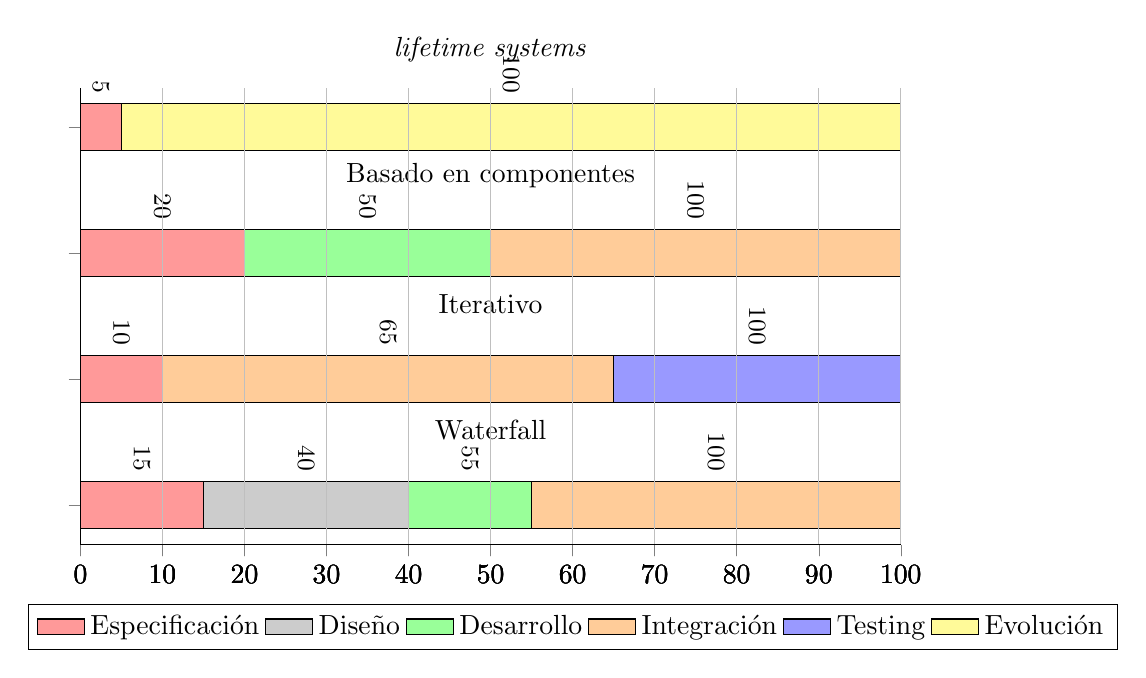
\begin{tikzpicture}
    \begin{axis}[testbar,title=Waterfall,legend style={area legend, at={(0.6,-0.75)}, anchor=north, legend columns=-1}] 
      \addplot[fill=red!40] coordinates{(15,0) };
      \addplot[fill=gray!40] coordinates{(25,0)};
      \addplot[fill=green!40] coordinates{(15,0) };
      \addplot[fill=orange!40] coordinates{(45,0)};
      \addplot[fill=blue!40] coordinates{(0,0) };
      \addplot[fill=yellow!40] coordinates{(0,0) };
      \legend{Especificación,Diseño,Desarrollo,Integración,Testing,Evolución}
    \end{axis}
    \begin{axis}[testbar,title = Iterativo] 
      \addplot[fill=red!40] coordinates{(10,2) };
      \addplot[fill=gray!40] coordinates{(0,0)};
      \addplot[fill=green!40] coordinates{(0,0) };
      \addplot[fill=orange!40] coordinates{(55,2)};
      \addplot[fill=blue!40] coordinates{(35,2) };
      \addplot[fill=yellow!40] coordinates{(0,0) };
    \end{axis}
    \begin{axis}[testbar,title = Basado en componentes] 
      \addplot[fill=red!40] coordinates{(20,4) }; % Especificación
      \addplot[fill=gray!40] coordinates{(0,0)}; % Diseño 
      \addplot[fill=green!40] coordinates{(30,4) }; % Desarrollo
      \addplot[fill=orange!40] coordinates{(50,4)}; % Integración
      \addplot[fill=blue!40] coordinates{(0,0) }; % Testing
      \addplot[fill=yellow!40] coordinates{(0,0) }; % Evolución
    \end{axis}
    \begin{axis}[testbar,title = \emph{lifetime systems}] 
      \addplot[fill=red!40] coordinates{(5,6) }; % Especificación
      \addplot[fill=gray!40] coordinates{(0,0)}; % Diseño 
      \addplot[fill=green!40] coordinates{(0,0) }; % Desarrollo
      \addplot[fill=orange!40] coordinates{(0,0)}; % Integración
      \addplot[fill=blue!40] coordinates{(0,0) }; % Testing
      \addplot[fill=yellow!40] coordinates{(95,6) }; % Evolución
    \end{axis}
  \end{tikzpicture}
  \label{fig:costemetodologia}
\end{figure}

Cuanto más tarde se encuentran errores en el Software, o más tarde se
hace un cambio de requisito, los cambios son más costosos. Comparando
el cambio en dos fases del ciclo de vida:

\begin{center}
\begin{tabular}{p{5cm} | p{7cm}}
  \textbf{Temprano} &   \textbf{Tardío} \\ \hline
  Cambio en la especificación. & Cambio en la especificación. \\
                    & Cambiar el código y la documentación. \\
                    & Probar el cambio. \\
                    & Testing. \\
                    & Instalación del producto en el cliente.
                                           
\end{tabular}  
\end{center}

A medida que pasa el tiempo, la cantidad de fallos que aparecen
aumentan debido al deterioro.

\section{El Software}
\label{sec:software}

Entre las características que se le atribuyen a un \emph{producto
  Software} encontramos:
\begin{itemize}[noitemsep]
\item Múltiples \textbf{programas}.
\item Archivos de \textbf{configuración}.
\item La \textbf{documentación} del sistema.
\item La documentación de \textbf{uso}.
\item Los \textbf{datos} del sistema.
\item \textbf{Actualización} de información.
\end{itemize}

El \textit{Software} se realiza para \textbf{clientes particulares} o
para el uso \textbf{general}. Esto está también relacionado con que
los productos de software sean \textbf{genéricos} o \textbf{a medida}.

Dependiendo del producto desarrollado, el software puede entrar en
categorías como: tiempo real, negocios, científico, emebido, PC, IA,
Web...

Los atributos de un \textbf{buen Software} varían según las perspectivas:
\index{buen Software}
\begin{center}
\begin{tabular}[h]{p{5cm} | p{5cm}}
  \textbf{Usuario} & \textbf{Desarrolador} \\ \hline
  Exactitud & Consistencia \\
  Confiabilidad & Comprensibilidad \\
  Eficiencia & Capacidad de ser probado \\
  Mantenibilidad & Compacidad \\
  Usabilidad & Compatibilidad \\
  Robustez & 
\end{tabular}  
\end{center}

\section{Procesos en el Software}
\label{sec:procesos}

Se entiende por \emph{proceso Software} un conjunto de \textbf{actividades y
  resultados} asociados a la producción de Software.

Este proceso se puede analizar desde diferentes perspectivas:
\begin{itemize}[noitemsep]
\item Flujo de \textbf{trabajo}.
\item Flujo de \textbf{datos}.
\item \textbf{Acción}.
\end{itemize}

Los modelos del \emph{ciclo de vida} del Software especifican las
fases del \emph{proceso de Software}. Hemos mencionado ya ejemplos en
la sección \ref{sec:costes}. Un modelo está compuesto de:
\begin{itemize}[noitemsep]
\item Descripción propia.
\item Reglas.
\item Recomendaciones (\emph{guías de estilo}).
\item Procesos (\emph{actividades a seguir}).
\end{itemize}

Estos \textbf{modelos} están orientados a resolver los retos de la ingeniería
del Software,\index{retos Software} muy relacionados con los atributos
del buen Software indicados en la sección \ref{sec:software}.

\begin{itemize}[noitemsep]
\item Heterogeneidad de plataformas.
\item Entrega más rápida.
\item Confianza.
\item Gastos en el Hardware/Software.
\item Adaptabilidad a nuevas tecnologías.
\item Usabilidad.
\item Mantenimiento.
\end{itemize}

\section{Ciclo de Vida}
\label{sec:cv}

\begin{center}
Qué hacer \textrightarrow Cómo hacerlo \textrightarrow Hacerlo
\textrightarrow Probarlo \textrightarrow Usarlo \textrightarrow
Mantenerlo
\end{center}

Para la realización del Software tendremos que tener en cuenta:
\begin{itemize}[noitemsep]
\item Escala.
\item Productividad.
\item Calidad (ISO).
  \begin{itemize}
  \item Funcionalidad, Fiabilidad, Usabilidad, Eficiencia,
    Manteniblidad, Portabilidad.
  \end{itemize}
\item Consistencia.
\item Tasa de cambio.
\end{itemize}

Este ciclo de vida se organiza en fases. De cada fase se obtendrá un
resultado que se utilizará en las siguientes fases. El \emph{ciclo de
  vida} del Software se enfoca en manejar la complejidad y el cambio
a lo largo de un proceso.

Existen distintos \emph{ciclos de vida}, nombrados como modelos
(sección \ref{sec:software}):
\begin{itemize}[noitemsep]
\item Informal.
\item Convencional.
\item Incremental.
\item Evolutivo.
\item Prototipado (puede ser incluido en los anteriores modelos).
\end{itemize}

Estos modelos tienen un equilibrio entre los siguietnes factores:
\begin{itemize}[noitemsep]
\item Velocidad de desarrollo.
\item Calidad.
\item Visibilidad.
\item Sobrecarga de gestión.
\item Exposición al riesgo.
\item Relaciones públicas.
\end{itemize}